\chapter{Diagnosis}%
\label{chap:diagnosis}%
\chapintro{This chapter is based on results published in~\cite{Lohmann_2008_wsfm}.}


\lettrine[findent=.2em,lines=2,nindent=-0.4em]{W}{e} introduced controllability as a fundamental correctness criterion for interacting service models. In the previous chapter, we presented behavioral constraints as a means to restrict the set of strategies to refine the analysis of a service. Controllability and the satisfaction of behavioral constraints can be automatically decided. The decision algorithm (cf.~\autoref{def:synthesis}) is constructive: If a strategy for a service exists, it can be synthesized and serves as a witness for controllability. If, however, the service is uncontrollable, no strategy exists and the algorithm neither returns a service nor any diagnosis information. In this chapter, we introduce a \emph{diagnosis framework for uncontrollable services}. In the next section, we present the various reasons which may make a service uncontrollable. In~\autoref{sect:diagnosis:counterexamples} and \autoref{sect:diagnosis:reduction}, we informally sketch how counterexamples for controllability (or witnesses for uncontrollability) may be presented to service modelers. \Autoref{diagnosis:sect:blacklists} is devoted to a formalization of the problem. The diagnosis algorithm is finally defined in \autoref{diagnosis:sect:algorithm} where we also discuss its implementation. \Autoref{sect:diagnosis:conclusion} concludes the chapter.





%%%%%%%%%%%%%%%%%%%%%%%%%%%%%%%%%%%%%%%%%%%%%%%%%%%%%%%%%%%%%%%%%%%%%%%%%%%%%%%
\section{Reasons for uncontrollability}\label{sect:diagnosis:reasons}
%%%%%%%%%%%%%%%%%%%%%%%%%%%%%%%%%%%%%%%%%%%%%%%%%%%%%%%%%%%%%%%%%%%%%%%%%%%%%%%

The presence of strategies (\ie,~clients, partner services, requestors, customers, etc.) is crucial for a service. To this end, controllability is a fundamental sanity check for services, and any other (behavioral) correctness criterion (\eg, stronger notions which also require the absence of livelocks in the composition) would likely further refine the set of strategies of a service. Controllability is defined as an extension of compatibility to open services, and we shall consider the requirements for compatibility when we reason about uncontrollability. A service is uncontrollable if there does not exist a composable service such that
\begin{niceenumerate}
\item every maximal run of the composition terminates in a final state,
\item the asynchronous message channels are bounded, and
\item the composition is responsive (\ie, no port is excluded from communication on infinite runs).
\end{niceenumerate}
An uncontrollable service has no strategy. Hence, we cannot analyze a concrete composition for the reasons which led to incompatible behavior. Therefore, we need to explain the absence of strategies by considering the service itself. In particular, we have to investigate the service's share of the incompatibility of the composition with \emph{any other} service. In the remainder of this section, we give examples how errors and design flaws of a single service can result in uncontrollability. We group these issues according to the three preceding requirements.




%%%%%%%%%%%%%%%%%%%%%%%%%%%%%%%%%%%%%%%%%%%%%%%%%%%%%%%%%%%%%%%%%%%%%%%%%%%%%%%
\subsection{Deadlocking run}

The algorithm suggested by \autoref{def:synthesis} removes all nodes which contain a deadlocking state; that is, a state which is neither final nor has a successor state in the composition of the service and the strategy overapproximation. Thereby, a state $[q,\mathcal{B}]$ has two components: state~$q$ representing the internal state of the service and a multiset~$\mathcal{B}$ modeling the pending asynchronous messages. These components help classify deadlocks.


\paragraph{Internal deadlock.}

First, the state $q$ of the service may be a deadlock itself; that is, $q$ is a nonfinal state without successors. We call such a state an \emph{internal deadlock}, because this deadlock is independent of a communication event. There are different reasons why a service may contain an internal deadlock:

\begin{niceitemize}
\item \emph{Design flaw.} An obvious reason for an internal deadlock is a classical design flaw. Although languages, such as \acronym{WS-BPEL}, have syntactical requirements to avoid modeling potential deadlocks, in graph-based languages, such as \acronym{BPMN}, it is possible to introduce deadlocks, for instance because of mismatching gateways. Such design flaws affect the control flow of a service and can be detected without taking the interaction into account. Classical control flow-oriented correctness notions such as soundness~\cite{Aalst_1998_jcsc} are, however, neither sufficient nor necessary for controllability of a service. We shall discuss this in \autoref{sect:diagnosis:counterexamples}.

\Autoref{diagnosis:fig:deadlock1} shows a service automaton, which contains an internal deadlock. The service nondeterministically decides whether to send an $a$-message or a $b$-message. The environment can only observe, but not influence this decision. As the deadlock cannot be avoided, the service is uncontrollable.

\item \emph{Service choreography.} Not every internal deadlock is the result of a modeling error. Another source of internal deadlocks can be the composition of several services in a service choreography. There, it is possible that the behavior of two participants is mutually exclusive leading to an internal deadlock.

\Autoref{diagnosis:fig:deadlock2} depicts two services whose composition has the same behavior as the service automaton in \autoref{diagnosis:fig:deadlock1}. The internal deadlock occurs, because the left service waits for a $d$-message and the right service waits for an $e$-message.

%%%%%%%%%%%%%%%%%%%%%%%%%%%%%%%%%%%%%%%%%%%%%%%%%%%%%%%%%%%%%%%%%%%%%%%%%%%%%%
\begin{figure}
\centering
\hfill
\subfigure[design flaw\label{diagnosis:fig:deadlock1}]{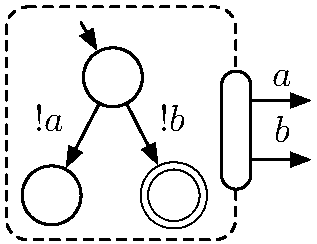
\includegraphics[scale=0.45]{diagnosis/deadlock1}} \hfill\hfill
\subfigure[deadlocking composition\label{diagnosis:fig:deadlock2}]{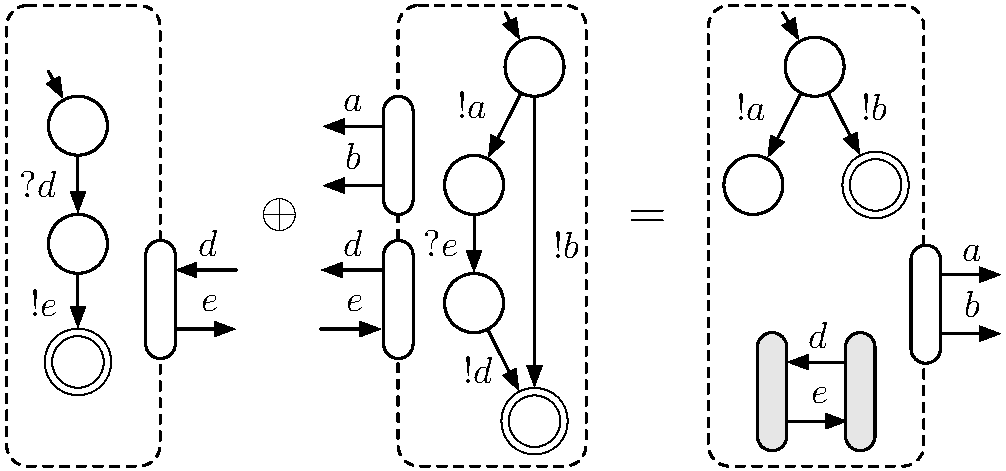
\includegraphics[scale=0.45]{diagnosis/deadlock2}}\hfill${}$
\caption{Uncontrollability caused by internal deadlocks.}
\end{figure}
%%%%%%%%%%%%%%%%%%%%%%%%%%%%%%%%%%%%%%%%%%%%%%%%%%%%%%%%%%%%%%%%%%%%%%%%%%%%%%

\item \emph{Behavioral constraint.} Another reason for internal deadlocks of a service is the consideration of a behavioral constraint $C$, cf.~\autoref{chap:validation}. In particular, final states of $A$ may become internal deadlocks in the product $A\otimes C$. These deadlocks are not design flaws, but model undesired situations. This may render a service uncontrollable as it may be impossible to satisfy the constraint.

\Autoref{validation:fig:product2} depicts a service automaton which contains the deadlocks $[q_{5},c_{2}]$ and $[q_{6},c_{2}]$ which were introduced by the constraint automaton depicted in \autoref{validation:fig:constraint5}. However, this service automaton is still controllable, because the deadlocks can be circumvented by the environment.
\end{niceitemize}


\paragraph{Covered final state.}

A \emph{covered final state} is a situation in which the control flow of $A$ reached a final state without successor state, but an asynchronous message sent to $A$ is still pending on an input channel. This message will never be received from the service. This may be negligible for generic acknowledgment messages, but an unreceived message is typically an undesired situation (\eg, if the message contains private or payment information). In addition, unexpected messages may lead to runtime errors during the execution of a \acronym{WS-BPEL} process. Again, there are many reasons for this problem:

%%%%%%%%%%%%%%%%%%%%%%%%%%%%%%%%%%%%%%%%%%%%%%%%%%%%%%%%%%%%%%%%%%%%%%%%%%%%%%
\begin{figure}
\centering
\subfigure[hidden choice\label{fig:un2}]{\makebox[0.33\textwidth]{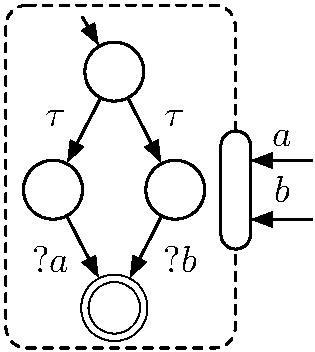
\includegraphics[scale=0.45]{diagnosis/nlc1}}}\hfill
\subfigure[conflicting receives\label{fig:un3}]{\makebox[0.33\textwidth]{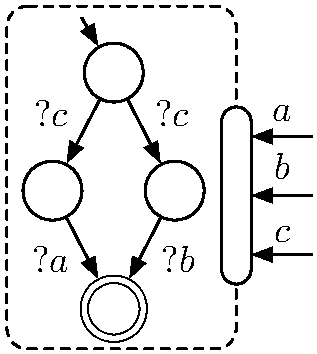
\includegraphics[scale=0.45]{diagnosis/nlc2}}}\hfill
\subfigure[delayed messages\label{fig:un4}]{\makebox[0.33\textwidth]{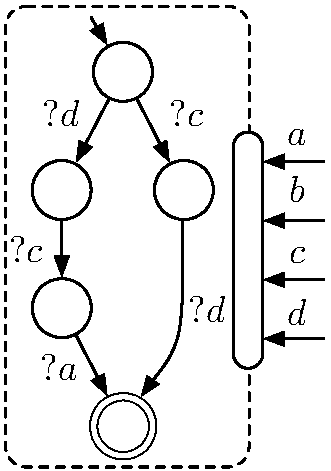
\includegraphics[scale=0.45]{diagnosis/nlc3}}}
\caption{Uncontrollability caused by covered final states.}\label{diagnosis:fig:sound}
\end{figure}
%%%%%%%%%%%%%%%%%%%%%%%%%%%%%%%%%%%%%%%%%%%%%%%%%%%%%%%%%%%%%%%%%%%%%%%%%%%%%%

\begin{niceitemize}
\item \emph{Hidden choice.} In case services implement business processes, data-dependent decisions (\eg, \acronym{WS-BPEL}'s \texttt{<if>} activity or a data-dependent gateway in \acronym{BPMN}) are common. Such a decision may be taken without explicitly informing the communication partner about the outcome. If this \emph{hidden choice} requires different reactions of the partner (\ie, the partner needs to send different messages), it cannot be guaranteed that each of these messages are received. 

Consider for example the service automaton in \autoref{fig:un2}, which nondeterministically chooses the left or the right branch. Depending on this internal choice, a partner has to send either an $a$-message or a $b$-message. The final marking is only reached, if the partner's ``guess'' was right. Otherwise, the ``wrong'' message keeps pending.

\item \emph{Conflicting receives.} If a service can reach a state in which more than one transition can receive the same message from an asynchronous channel or synchronize with the same event, these transitions are \emph{conflicting receives}~\cite{standard_bpel}. The decision which branch to take, can neither be influenced nor observed by a partner yielding a hidden choice situation. Execution languages like \acronym{WS-BPEL} treat conflicting receives as runtime faults, but similar to internal deadlocks, we do not want to forbid such situations in the first place. Instead, we want to investigate whether these problems are the original reason a service is uncontrollable.

The initial state of the service automaton in~\autoref{fig:un3} models a conflicting receive situation. After sending a $c$-message, a partner has to  send either an $a$-message or a $b$-message to the service. If the wrong choice is made, the message keeps pending on the input channel. This eventually yields a covered final state.

\item \emph{Delayed messages.} Service automata support asynchronous message exchange: messages can keep pending on a channel and overtake one other. Therefore, a partner has only limited control over a service, because after sending a message, a partner cannot observe whether this message was already received or whether it is still pending on the channel. Again, this can result in a ``hidden choice'' situation.

An example is given in \autoref{fig:un4}. The order in which the $c$-message and the $d$-message are sent to the service does not determine the order in which these messages are received and, consequently, which branch is taken. However, an $a$-message is only received if the left branch is taken and remains pending otherwise.
\end{niceitemize}

Covered final states can be seen as a ``visible symptom'' of uncontrollability rather than an original fault. For instance, there can be an arbitrary number of transitions leading from a hidden choice to covered final state. This makes the detection of the reasons which actually led to uncontrollability nontrivial.




%%%%%%%%%%%%%%%%%%%%%%%%%%%%%%%%%%%%%%%%%%%%%%%%%%%%%%%%%%%%%%%%%%%%%%%%%%%%%%%
\subsection{Exceeded message bound}

Beside the requirement that the message channels must be empty in a final state, compatibility demands that the message channels never exceed a given bound $k$. Consequently, also this message bound $k$ influences in \autoref{def:synthesis} the removal of states of $\TS^{0}(A)$ when constructing $\TS^{1}_{k}(A)$. There are two situations to consider:

%%%%%%%%%%%%%%%%%%%%%%%%%%%%%%%%%%%%%%%%%%%%%%%%%%%%%%%%%%%%%%%%%%%%%%%%%%%%%%
\begin{figure}
\centering
\subfigure[unbounded channel\label{fig:un6}]{\makebox[0.5\textwidth]{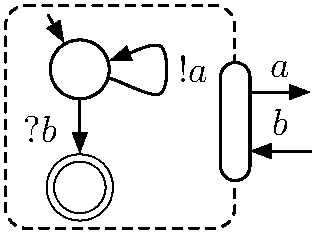
\includegraphics[scale=0.45]{diagnosis/mb1}}}\hfill
\subfigure[channel bound $k>1$\label{fig:un7}]{\makebox[0.5\textwidth]{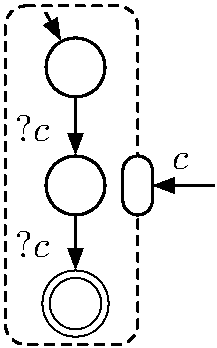
\includegraphics[scale=0.45]{diagnosis/mb2}}}
\caption{Uncontrollability caused by message bound excess ($k=1$).}
\end{figure}
%%%%%%%%%%%%%%%%%%%%%%%%%%%%%%%%%%%%%%%%%%%%%%%%%%%%%%%%%%%%%%%%%%%%%%%%%%%%%%


\paragraph{Unbounded communication.}

If a message channel is unbounded (\eg, caused by a loop of the service in which it sends messages without waiting for acknowledgements), then obviously no partner can exist such that the composition is $k$-bounded. \Autoref{fig:un6} shows an example where the output channel $a$ is unbounded. Even if the environment sends a $b$-message to this service, its receipt can be postponed arbitrarily.


\paragraph{Inadequate message bound.}

If a service is $k$-controllable for a message bound $k\in\mathds{N}^+$, it is also $l$-controllable for any bound $l>k$. The converse does not hold: \Autoref{fig:un7} shows a service which is $2$-controllable, but not $1$-controllable, because the receipt of the first $c$-message cannot be enforced before sending a second $c$-message. This results in a state where two $c$-messages are pending and the message bound is violated. Thus, even if a message bound exists for a service, this service may be considered $k$-uncontrollable if the message bound~$k$ chosen for analysis is too small. Again, we do not want to rely on the underlying infrastructure, which may enforce a message bound by discarding messages, but to treat exceeded message bounds as a design flaw we want to diagnose. Note that the message bound can be violated for output message channels (cf.~\autoref{fig:un6}) and input message channels~(cf.~\autoref{fig:un7}).




%%%%%%%%%%%%%%%%%%%%%%%%%%%%%%%%%%%%%%%%%%%%%%%%%%%%%%%%%%%%%%%%%%%%%%%%%%%%%%%
\subsection{Unresponsiveness}

\Autoref{def:synthesis} was only defined for responsive service automata. Similar to internal deadlocks, unresponsive behavior does not necessarily result in uncontrollability. Instead of restricting diagnosis to responsive services, it should be investigated whether it is the original reason of uncontrollability of a service.

%%%%%%%%%%%%%%%%%%%%%%%%%%%%%%%%%%%%%%%%%%%%%%%%%%%%%%%%%%%%%%%%%%%%%%%%%%%%%%
\begin{figure}
\centering
\subfigure[internal livelock\label{diagnosis:fig:livelock1}]{\makebox[0.5\textwidth]{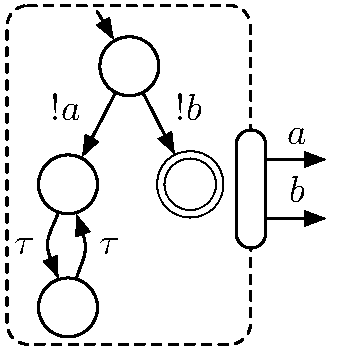
\includegraphics[scale=0.45]{diagnosis/livelock}}}\hfill
\subfigure[unresponsive communication\label{diagnosis:fig:livelock2}]{\makebox[0.5\textwidth]{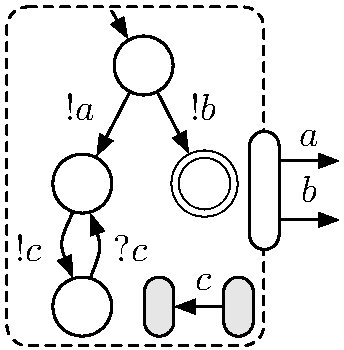
\includegraphics[scale=0.45]{diagnosis/livelock2}}}
\caption{Uncontrollability caused by unresponsive behavior.}
\end{figure}
%%%%%%%%%%%%%%%%%%%%%%%%%%%%%%%%%%%%%%%%%%%%%%%%%%%%%%%%%%%%%%%%%%%%%%%%%%%%%%


\paragraph{Internal livelock.}

A service can make a service composition unresponsive if it continuously changes its state without interaction with all ports environment and without reaching a final state. Such diverging behavior is an \emph{internal livelock} and can be checked locally similar to internal deadlocks. \Autoref{diagnosis:fig:livelock1} shows an example. An internal livelock can also model the closed communication between two implemented ports. Consider the service automaton \autoref{diagnosis:fig:livelock2}. Once this service sends an $a$-message, the port $[\emptyset,\{a,b\}]$ is excluded from further communication.

\medskip

The issues presented in this section are the original problems which can make a service uncontrollable. Deadlocks and message bound violations\,---\,\autoref{def:synthesis} only takes responsive service automata into account\,---\, yield to the deletion of such states. This deletion can introduce other deadlocks. These states usually give no further information on the original reasons which make a service uncontrollable. To this end, we focus on the detection of internal deadlocks, covered final states, and message bound violations. In addition, we have to consider unresponsive services; that is, we need to detect internal livelocks as reasons for uncontrollability.





%%%%%%%%%%%%%%%%%%%%%%%%%%%%%%%%%%%%%%%%%%%%%%%%%%%%%%%%%%%%%%%%%%%%%%%%%%%%%%%
\section{Counterexamples for controllability}
\label{sect:diagnosis:counterexamples}
%%%%%%%%%%%%%%%%%%%%%%%%%%%%%%%%%%%%%%%%%%%%%%%%%%%%%%%%%%%%%%%%%%%%%%%%%%%%%%%

As motivated the synthesis algorithm gives no information on the reasons which make a service uncontrollable. Before we elaborate on how diagnosis information could be presented, we study a related diagnosis approach.




%%%%%%%%%%%%%%%%%%%%%%%%%%%%%%%%%%%%%%%%%%%%%%%%%%%%%%%%%%%%%%%%%%%%%%%%%%%%%%
\subsection*{Relationship to soundness}

Controllability of a service model has a close relationship to soundness in the area of workflow models~\cite{Aalst_1998_jcsc}. However, existing diagnosis techniques for unsound workflow models~\cite{VerbeekBA_2001_tcj} are not applicable to diagnose uncontrollability, because the service's interaction with the environment has to be taken into account.

For a controllable service $A$ there exists service $B$ such that $A\oplus B$ are compatible. Compatibility is closely related to \emph{soundness}~\cite{Aalst_1998_jcsc}. In fact, soundness is more strict because it rules out activities which are never executed as well as livelocks. For soundness, an elaborate diagnosis algorithm exists~\cite{VerbeekBA_2001_tcj}, which exploits several properties of the soundness criterion to avoid a complex state space exploration whenever possible. For example, soundness can be expressed in terms of two simpler Petri net properties, namely \emph{liveness} and \emph{boundedness}. An unsound workflow net fails one of these tests. This result can be used to give detailed diagnosis information. In addition, several simple necessary or sufficient criteria for soundness can be checked before liveness and boundedness checks. For example, certain net classes such as \emph{free choice Petri nets}~\cite{DeselE_1995} allow for efficient analysis algorithms. However, this diagnosis approach cannot be adapted to diagnose the reasons of why a service automaton is uncontrollable.

First, a sound control flow does not imply controllability, and vice versa. For example, the control flow of the controllable service automaton in \autoref{validation:fig:product2} is not sound (due to internal deadlocks), and the uncontrollable service automata in \autoref{diagnosis:fig:sound} all have a sound control flow. Similarly, weaker criteria such as \emph{relaxed soundness} or \emph{non-controllable choice robustness}~\cite{DehnertA_2004_ijcis} are not applicable. The latter, for example, assumes that the environment can completely observe the service's state, whereas the internal state of a service can only be guessed from observations on the interface (to this end, a state of the synthesized strategy contains of a \emph{set} of states of the service together with its asynchronous interface).

Second, controllability is not a local, but a global criterion: only under restricted preconditions controllability can be decomposed~\cite{Lohmann_2008_awpn}. The previous section shows that there are multiple reasons that can make a service uncontrollable. Unfortunately, these examples cannot serve as antipatterns. Intuitively, every service that contains a bad scenario such as a hidden choice or an internal deadlock, can be extended such that the problem is either resolved or avoided in the first place (cf.~\autoref{fig:diagnosis:antipatterns}). To this end, it is impossible to consider only a fraction of the states of a service and make a statement about the correctness of the service. Therefore, only limited necessary or sufficient structural criteria for (un)controllability exist~\cite{Richter_2001_sa,Martens_2003_phd}. Finally, structural results like the invariant calculus~\cite{LautenbachR_1994_atpn} for Petri nets are not applicable, because these techniques do not take the interface into account.

%%%%%%%%%%%%%%%%%%%%%%%%%%%%%%%%%%%%%%%%%%%%%%%%%%%%%%%%%%%%%%%%%%%%%%%%%%%%%%
\begin{figure}
\centering
\subfigure[resolve problem\label{fig:diagnosis:resolve}]{\makebox[0.5\textwidth]{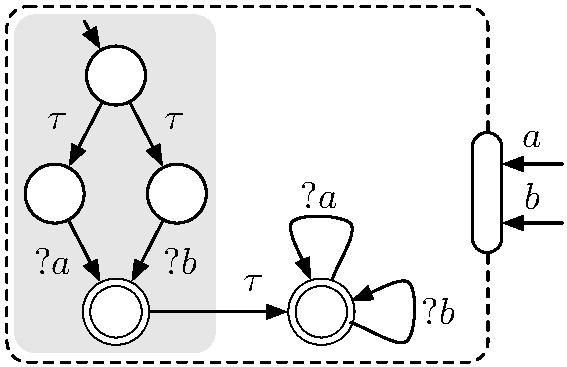
\includegraphics[scale=0.45]{diagnosis/nonlocal2}}}\hfill
\subfigure[avoid problem\label{fig:diagnosis:avoid}]{\makebox[0.5\textwidth]{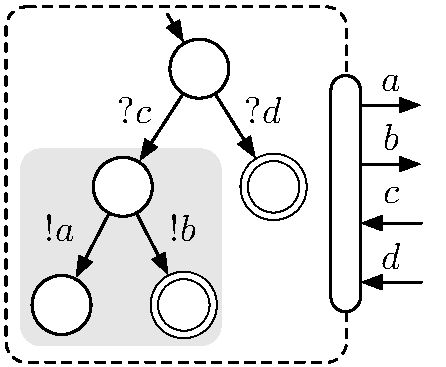
\includegraphics[scale=0.45]{diagnosis/nonlocal1}}}
\caption{Uncontrollability cannot be checked locally using antipatterns (shaded gray): pending messages can be received later~(a) and internal deadlocks can be avoided (b).}
\label{fig:diagnosis:antipatterns}
\end{figure}
%%%%%%%%%%%%%%%%%%%%%%%%%%%%%%%%%%%%%%%%%%%%%%%%%%%%%%%%%%%%%%%%%%%%%%%%%%%%%%




%%%%%%%%%%%%%%%%%%%%%%%%%%%%%%%%%%%%%%%%%%%%%%%%%%%%%%%%%%%%%%%%%%%%%%%%%%%%%%
\subsection*{Counterexamples}

In case structural methods are not applicable or can only give partial information on the correctness of a system, the \emph{behavior} of the system (\ie, its state space) needs to be analyzed. The ability to generate \emph{counterexamples} greatly boosted the acceptance of model checking~\cite{ClarkeGD_1999_book} in the field of computer-aided verification. If a model does not meet a given specification, model checking techniques automatically provide such a counterexample. For the modeler, this is a useful artifact (\eg, a deadlock trace) to understand the reasons \emph{why} the model contains an error, how it is reached, and how to fix the model. Likewise, \emph{witnesses} are useful means to prove that a system satisfies certain properties.

To find a counterexample for controllability is a nontrivial task because of the criterion's nature. Controllability is ``proved'' by constructing a witness: $A$ is $k$-controllable iff there \emph{exists} some service $B$ such that the composition $A\oplus B$ is $k$-compatible. In other words, $B$ can be seen as a counterexample for $A$'s \emph{un}controllability. If $A$ is not controllable, we can only conclude that \emph{no} such service exists, and hence cannot provide a counterexample which can be used to find out, which of the various problems we described in the previous section rendered the service uncontrollable.

The algorithm to decide controllability (cf. \autoref{def:synthesis}) overapproximates a strategy for $A$ and then iteratively removes states of this overapproximation which will not be part of any strategy of $A$. If $A$ is uncontrollable, all states will be eventually deleted. In the remainder of this section, we elaborate how a counterexample for $A$'s controllability (or a witness for $A$'s uncontrollability) should be shaped to support to locate and to understand the problems that lead to uncontrollability. In the next two sections, we then define an algorithm to use information why states are deleted from $\TS^{0}(A)$ and $\TS_{k}^{j}(A)$ to give diagnosis information for an uncontrollable service $A$.

As a motivation for the desired style of diagnosis information, consider again the service in \autoref{fig:un3}. We already described informally why this service is uncontrollable: 
\begin{quote}
After sending a $c$-message, a partner has to send either an $a$-message or a $b$-message to the service. If the wrong choice is made, the message keeps pending on the input channel. This eventually yields a covered final state.
\end{quote}

Let us analyze this informal description of why the service is uncontrollable. It contains:
\begin{labeling}{(\acronym{C})}
\item[(\acronym{I})] an indisputable initial part (``after sending a $c$-message'') which describes the communication between the service and a possible interaction partner,
\item[(\acronym{C})] a description of possible continuations (``a partner has to  send either an $a$-message or a $b$-message'') which are derived from the service's control flow, and
\item[(\acronym{P})] the problem which ultimately hinders a partner achieve compatibility of the composition (``If the wrong choice is made, the message keeps pending on the input channel. This eventually yields a covered final marking.'').
\end{labeling}

Before we explain the parts, we need to introduce \emph{waitstates}, which model situations in $\TS_0$ which can only be left with the help of the environment.

%%%%%%%%%%%%%%%%%%%%%%%%%%%%%%%%%%%%%%%%%%%%%%%%%%%%%%%%%%%%%%%%%%%%%%%%%%%%%%
\begin{definition}{Waitstate}
Let $A$ be a service automaton. The pair $[q,\mathcal{B}]\in Q_A\times\Bags(\M_a)$ is a \define{waitstate} if, for all $q\in Q_{A}$ and $e\in\E$, \smash{$q\xrightarrow{e}_A q'$} implies (1) $e\in {?\E}$ and $\mathcal{B}(\M(e))=0$ or (2) $e\in{\sync\E}$. This waitstate can be \define{resolved} by (1)~sending an asynchronous message $e$ to $A$ or by (2) synchronizing with $A$ via channel $e$, respectively.
\end{definition}
%%%%%%%%%%%%%%%%%%%%%%%%%%%%%%%%%%%%%%%%%%%%%%%%%%%%%%%%%%%%%%%%%%%%%%%%%%%%%%

A waitstate is a situation the service automaton $A$ cannot leave without communication with the environment; that is, an asynchronous message needs to be received or a synchronization with the environment is required. The notion of waitstates will be used to define the (\acronym{I}), (\acronym{C}), and (\acronym{P}) parts of the previous description. The initial part (\acronym{I}) consists of communication steps which are necessary to resolve a waitstate and which would also be taken by partners who \emph{know} the outcome of the service's decision in advance. Sending a $c$-message is not source of the problem, because this message \emph{will} be received by the service. In contrast, after sending an $a$-message, any continuation~(\acronym{C}) \emph{can} lead to a situation where reaching a final marking is not any more guaranteed. Finally, the possible problem which can occur after sending either message is described (\acronym{P}). This subtle distinction between indisputable ``safe'' interactions and problematic ``unsafe'' interactions is crucial to construct an artifact that can serve as counterexample.

In the following, we generalize this approach and elaborate the required information to define an algorithm which automatically derives such diagnosis results for an uncontrollable service $A$ consisting of these three parts:
\begin{labeling}{(\acronym{C})}
\item[(\acronym{I})] From the strategy overapproximation $\TS^{0}(A)$, we define a maximal subgraph $\TS^{0*}_{k}(A)$ such that the composition $A\oplus \TS^{0*}_{k}(A)$ is free of \emph{bad states}. A state is considered bad if it contains an internal deadlock, a covered final state, an exceeded message bound, or an internal livelock.

\item[(\acronym{C})] The subgraph $\TS^{0*}_{k}(A)$ is not a strategy of $A$, because its nodes contain waitstates which are not resolved in $\TS^{0*}_{k}(A)$, because the respective edge to a successor is missing. When these waitstates are resolved by sending messages to or by synchronizing with $A$, the composition may reach a state from which a bad state cannot be avoided any more. Therefore, in the second part of the diagnosis result, each unresolved waitstate is described including a communication trace from the initial state to the state containing this waitstate.

\item[(\acronym{P})] Finally, we give detailed information how the resolution of the waitstate can reach a bad state. For each problem, witness paths to the problematic situation or pointers to the structure of $A$ are given to locate the problem.
\end{labeling}

\Autoref{fig:diagnosis:counterexample} illustrates the overall shape of a counterexample for controllability. It is a subgraph of $\TS^{0}$ from which all blacklisted bad states~(\acronym{P}) are removed. The actual diagnosis information can then derived from those waitstates from which a transition to blacklisted states is inevitable~(\acronym{C}). The initial part~(\acronym{I}) may be empty in case a bad situation (\ie, an internal deadlock, etc.) can be reached from the initial state without interaction, cf.~\autoref{diagnosis:fig:deadlock1}. The final diagnosis algorithm will treat this case separately.

%%%%%%%%%%%%%%%%%%%%%%%%%%%%%%%%%%%%%%%%%%%%%%%%%%%%%%%%%%%%%%%%%%%%%%%%%%%%%%
\begin{figure}
\centering
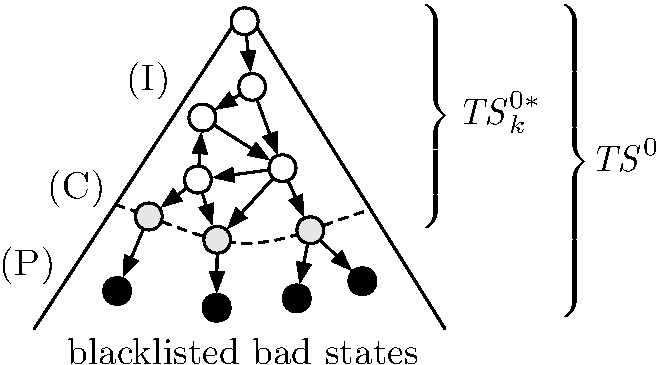
\includegraphics[scale=0.45]{diagnosis/counterexample}
\caption{A counterexample for controllability consists of an initial part (\acronym{I}), possible continuations (\acronym{C}), and resulting problems~(\acronym{P}). The subgraph $\TS^{0*}_k$ is defined using blacklists.}
\label{fig:diagnosis:counterexample}
\end{figure}
%%%%%%%%%%%%%%%%%%%%%%%%%%%%%%%%%%%%%%%%%%%%%%%%%%%%%%%%%%%%%%%%%%%%%%%%%%%%%%





%%%%%%%%%%%%%%%%%%%%%%%%%%%%%%%%%%%%%%%%%%%%%%%%%%%%%%%%%%%%%%%%%%%%%%%%%%%%%%%
\section{An overapproximation of a counterexample}
\label{sect:diagnosis:reduction}
%%%%%%%%%%%%%%%%%%%%%%%%%%%%%%%%%%%%%%%%%%%%%%%%%%%%%%%%%%%%%%%%%%%%%%%%%%%%%%%

The counterexample we sketched in the previous section is based on a subgraph of the strategy overapproximation $\TS^{0}(A)$ from \autoref{def:synthesis}. Before we go into details on how to derive this subgraph, we have to make sure that the counterexample we construct does not contain unnecessary parts.

\Autoref{def:synthesis} aims at synthesizing a most-permissive strategy for a service $A$. The algorithm achieves this by first generating the behavior of \emph{any} service communicating with $A$. This leads to several bad states in the composition $\TS^{0}(A)\oplus A$, which are iteratively removed. Only by starting out with a maximal overapproximation, most-permissiveness is guaranteed.

In case a service is uncontrollable, every state is eventually considered bad. However, not every bad state can be used to derive diagnosis information. To explain the reasons which lead to uncontrollability, the overapproximation should contain as few states as possible. In particular, messages should be only sent if they can resolve a waitstate. Likewise, receive and synchronization events should only occur if they are really possible. If we construct an overapproximation in this fashion (\ie, the construction of every state has a reason), we can derive concrete diagnosis information from bad states.

Although a smaller overapproximation is not suitable to construct a most-permissive strategy, it can dramatically speed up the synthesis of an arbitrary strategy. \citet{Weinberg_2008_wsfm} defined several on-the-fly reduction rules to find compact strategies. These strategies can be used in case only the \emph{existence} of a strategy is of interest rather than a complete characterization of all strategies satisfying the constraint.

We use two reduction rules from~\cite{Weinberg_2008_wsfm}: The first rule (called ``activated events'') avoids synthesizing unreachable behavior and only sends messages to resolve waitstates. The second rule (called ``receive before send'') prioritizes receiving events before sending events. The result is a smaller overapproximation. We adjust \autoref{def:synthesis} as follows.


%%%%%%%%%%%%%%%%%%%%%%%%%%%%%%%%%%%%%%%%%%%%%%%%%%%%%%%%%%%%%%%%%%%%%%%%%%%%%%
\begin{definition}{Reduced strategy synthesis}
\label{def:synthesisreduced}%
Let $A=[Q_{A},q_{0_{A}},{\shortrightarrow}_{A},\Omega_{A},\mathcal{P}_{A}]$ be an open finite state service automaton with $\mathcal{P}_{A}=\{[I_{1},O_{1}],\ldots,[I_{n},O_{n}]\}$. We define the open service automaton $\TS^{0}_{\textit{red}}(A)=[Q,q_{0},{\shortrightarrow},\Omega,\mathcal{P}]$ with $\mathcal{P}=\{[O,I]\mid [I,O]�\in \mathcal{P}_{A} \cap ( \M_{\mathcal{P}_{A}}^\open\times \M_{\mathcal{P}_{A}}^\open )\}$ and $Q$, $q_{0}$, ${\shortrightarrow}$, and $\Omega$ inductively as follows:
\begin{myitemize}
\item Base: Let $q_{0}:=\closure_{A}(\{[q_{0_{A}},\emptymset]\})$. Then $q_{0}\in Q$.
\item Step: For all $q\in Q$ and $m\in\M$:
\begin{enumerate}
\item If ${!m}\in \E_{\mathcal{P}}$ and $[q_{1},\mathcal{B}]\in q$ with (i) $q_{1}\xrightarrow{?m}_{A}q_{2}$, (ii) $\mathcal{B}(m)=0$, and (iii) $\mathcal{B}(m')=0$ for all $m'\in \bigcup_{j=1}^{n} I_{j}$, let $q':=\closure_{A}(\{ [q_{A},\mathcal{B}+[m]] \mid [q_{A},\mathcal{B}] \in q \})$.
Then $q'\in Q$ and \smash{$q\xrightarrow{!m}q'$}.
\item If ${?m}\in \E_{\mathcal{P}}$, let $q':=\closure_{A}(\{ [q_{A},\mathcal{B}] \mid [q_{A},\mathcal{B}+[m]] \in q \})$.\\ If $q'\neq\emptyset$, then $q'\in Q$ and $q\xrightarrow{?m}q'$.
\item If $\sync m\in \E_{\mathcal{P}}$, let $q':=\closure_{A}(\{ [q_{A}',\mathcal{B}] \mid [q_{A},\mathcal{B}] \in q$ $\wedge$ \mbox{$q_{A}\xrightarrow{\sync m}_{A}q_{A}'$}$\})$. If $q'\neq\emptyset$, then $q'\in Q$ and $q\xrightarrow{\sync m}q'$.
\end{enumerate}
\item We define $\Omega:=\{ q \in Q�\mid q \cap (\Omega_{A}\times\{\emptymset\}) \neq \emptyset \}$.
\end{myitemize}
\end{definition}
%%%%%%%%%%%%%%%%%%%%%%%%%%%%%%%%%%%%%%%%%%%%%%%%%%%%%%%%%%%%%%%%%%%%%%%%%%%%%%

From $\TS^{0}_\mathit{red}(A)$, we proceed as in \autoref{def:synthesis} by iteratively removing states where the message bound is violated or which contain deadlocks, yielding $\TS_{k_\mathit{red}}(A)$. Compared to \autoref{def:synthesis}, the following adjustments have been made:
\begin{niceitemize}
\item An asynchronous message $m$ is only sent if it resolves a waitstate and if no receiving event is possible. This is expressed by adding to (1.) the requirement that the state $q$ must contain a state $[q_{1},\mathcal{B}]$ in which (i) message $m$ can be received by $A$, (ii) that no message is pending on the input channel $m$, and that (iii) also all output channels are empty in state~$[q_{1},\mathcal{B}]$.
\item Asynchronous receive events and synchronization events are only added if they are actually possible. In \autoref{def:synthesis}, state $q'$ and transition \smash{$q\xrightarrow{?m}q'$} were added even if there exists no state $[q^{*},\mathcal{B}]\in q$ with $\mathcal{B}(m)>0$. In this case, $q'=\emptyset$ (cf.~\autoref{fig:mpp}). The same effect can occur if a synchronization event is not possible. Hence, the reduced strategy only contains states~$q$ with $q\neq\emptyset$.
\item Finally, responsiveness of $A$ is not required. If $A$ is uncontrollable, because it is unresponsive, the diagnosis algorithm should report this.
\end{niceitemize}

The first adjustment ensures that every sending event has a ``reason'', namely the resolution of a waitstate. The second adjustment rules out unreachable behavior in the overapproximation, which does not help to diagnose reasons for uncontrollability. As discussed earlier, the application of the reduction rules do not synthesize a most-permissive strategy and is therefore not applicable during the calculation of an operating guideline. However, \autoref{def:synthesisreduced} does synthesize a strategy if and only if the service is controllable~\cite{Weinberg_2008_wsfm}.

%%%%%%%%%%%%%%%%%%%%%%%%%%%%%%%%%%%%%%%%%%%%%%%%%%%%%%%%%%%%%%%%%%%%%%%%%%%%%%
\begin{proposition}{Reduced strategy proves controllability~\cite{Weinberg_2008_wsfm}}
$A$ is $k$-controllable iff \smash{$Q_{\TS_{k_\mathit{red}}(A)}\neq\emptyset$}.
\end{proposition}
%%%%%%%%%%%%%%%%%%%%%%%%%%%%%%%%%%%%%%%%%%%%%%%%%%%%%%%%%%%%%%%%%%%%%%%%%%%%%%

To put it differently: \Autoref{def:synthesisreduced} preserves the reasons for uncontrollability and $\TS^{0}_\mathit{red}(A)$ can be used as an overapproximation for a counterexample rather than $\TS^{0}(A)$.


\paragraph{Example.}

\autoref{fig:diagnosis:reduced} depicts a comparison between a most-permissive strategy and a reduced synthesized strategy. In the reduced strategy, the invoice ($i$) is only sent to resolve the waitstate $[q_{4},\emptymset]$.

%%%%%%%%%%%%%%%%%%%%%%%%%%%%%%%%%%%%%%%%%%%%%%%%%%%%%%%%%%%%%%%%%%%%%%%%%%%%%%
\begin{figure}[t]
\centering
\subfigure[$\TS_{1}(A_{Buy})$]{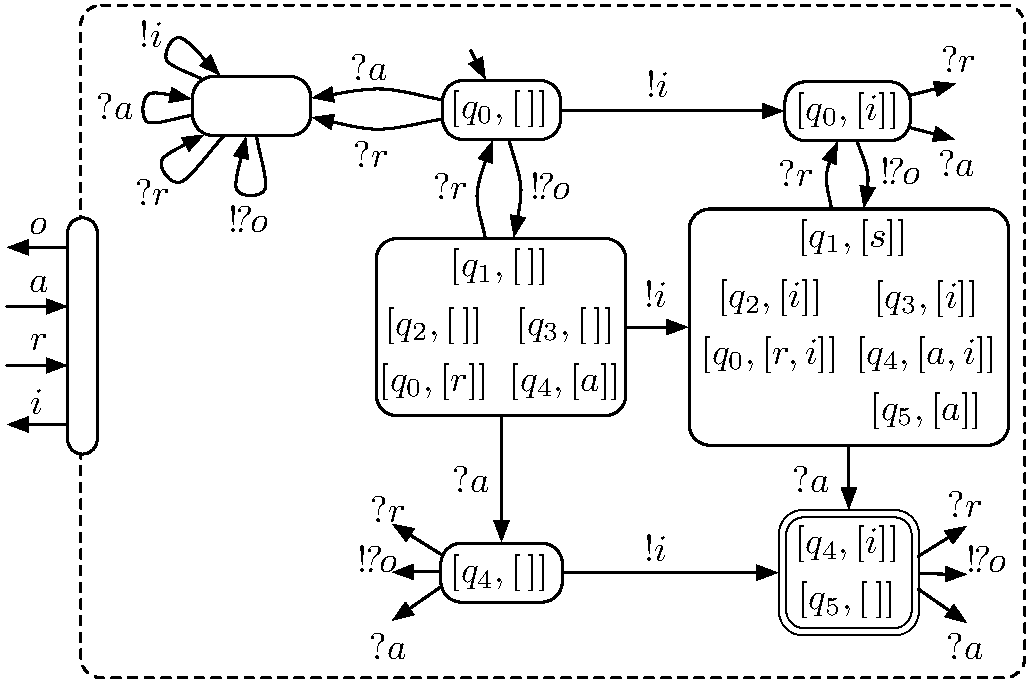
\includegraphics[scale=0.45]{background/running_mpp}}\hfill
\subfigure[$\TS_{1_\mathit{red}}(A_{Buy})$]{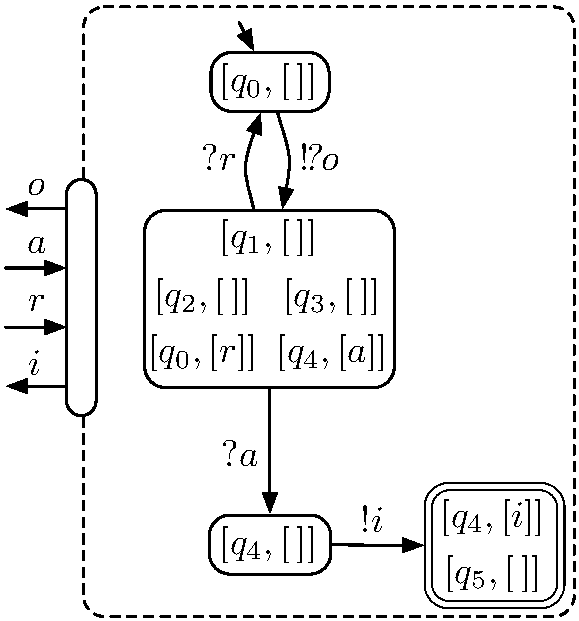
\includegraphics[scale=0.45]{diagnosis/reduced}}\caption{A most-permissive strategy (a) and the reduced synthesized strategy (b) for the buyer service from Fig.~\ref{fig:Asell}.}
\label{fig:diagnosis:reduced}
\end{figure}
%%%%%%%%%%%%%%%%%%%%%%%%%%%%%%%%%%%%%%%%%%%%%%%%%%%%%%%%%%%%%%%%%%%%%%%%%%%%%%





%%%%%%%%%%%%%%%%%%%%%%%%%%%%%%%%%%%%%%%%%%%%%%%%%%%%%%%%%%%%%%%%%%%%%%%%%%%%%%%
\section{Blacklist-based diagnosis}\label{diagnosis:sect:blacklists}
%%%%%%%%%%%%%%%%%%%%%%%%%%%%%%%%%%%%%%%%%%%%%%%%%%%%%%%%%%%%%%%%%%%%%%%%%%%%%%%

To derive diagnosis information\,---\,our counterexample demonstrating uncontrollability\,---\,, we first need a criterion to decide for each state of $\TS^{0}_\mathit{red}(A)$ whether it is a state of the subgraph $\TS^{0*}_{k}(A)$, too. We already motivated that $\TS^{0*}_{k}(A)$ should not contain bad states. Thus, for each problem, we define a \emph{blacklist} which contains such bad states. With these blacklists, we then can define the subgraph $\TS^{0*}_{k}(A)$.

For some bad states, it is also possible to characterize states which eventually \emph{will} be bad. For instance, a state whose successors are all internal deadlocks can likewise be considered bad, because once this state is reached, the service will eventually deadlock. This not only reduces the size of $\TS^{0*}_{k}(A)$, but also the length of the witness paths. Whereas the \emph{early detection} of internal deadlocks is straightforward and already exploited in the setting of behavioral constraints (cf.~\autoref{sect:validation_implementation}), the early detection of covered final states is more challenging. In particular, a covered final marking does not need to occur immediately after a hidden choice, but can occur many communication steps later.

In addition, we define a witness for each problem. A witness is an artifact which can help to locate the parts of the uncontrollable service that cause the problem (\eg, the transitions modeling a hidden choice or an internal deadlock state).




%%%%%%%%%%%%%%%%%%%%%%%%%%%%%%%%%%%%%%%%%%%%%%%%%%%%%%%%%%%%%%%%%%%%%%%%%%%%%%%
\subsection*{Blacklist for deadlocking and livelocking control flow}

Internal deadlocks and internal livelocks (\ie, unresponsive behavior) are problems that can be detected by analyzing the service in isolation. An internal livelock is a nonempty terminal strongly connected set of states of $A$, which neither contains a final state nor an open communication event. Because every internal deadlock is a (trivial) internal livelock, we can define a combined blacklist for internal deadlocks and internal livelocks as follows.

%%%%%%%%%%%%%%%%%%%%%%%%%%%%%%%%%%%%%%%%%%%%%%%%%%%%%%%%%%%%%%%%%%%%%%%%%%%%%%
\begin{definition}{Blacklist for internal deadlocks and livelocks}
We define the set of inevitable internal deadlocks of $A$, $Q_{DL}\subseteq Q_{A}$, to be the smallest set fulfilling:
\begin{myitemize}
\item If $q\not\xrightarrow{}_{A}$ and $q\notin\Omega_{A}$, then $q\in Q_{DL}$.
\item If $q\notin\Omega_{A}$ and, for all $x\in\E$, $q\xrightarrow{x}_{A} q'$ implies $q'\in Q_{DL}$, then $q\in Q_{DL}$.
\end{myitemize}

A set of states $Q_{LL}\subseteq Q_A$ is a livelock iff $Q_{LL}$ is a terminal strongly connected component of $A$ and $q\notin\Omega_{A}$ and $\lab(q)=\emptyset$, for all $q\in Q_{LL}$. Let $\mathcal{LL}$ be the set of all internal livelocks of $A$.

From these sets, define the \define{blacklist for internal deadlocks and internal livelocks} as $\bl_\mathit{DLL}:=\{q\in Q_{\TS^{0}_\mathit{red}(A)}�\mid q \cap ((Q_{DL}\cup \bigcup \mathcal{LL}) �\times \Bags(\M))�\neq \emptyset\}$. For each blacklisted state $q\in\bl_\mathit{DLL}$, define the witness $W_{DLL}(q):=\{q_d\in (Q_{DL} \cup\bigcup
\mathcal{LL})\mid [q_d,\mathcal{B}]\in q\}$.
\end{definition}
%%%%%%%%%%%%%%%%%%%%%%%%%%%%%%%%%%%%%%%%%%%%%%%%%%%%%%%%%%%%%%%%%%%%%%%%%%%%%%

We not only blacklist states which contain an internal deadlock, but also states which contain a state from which an internal deadlock will be eventually reached. For a blacklisted state $q$, the witness $W_{DLL}(q)$ is the set of all (inevitable) internal deadlocks and the internal livelocks in~$q$.




%%%%%%%%%%%%%%%%%%%%%%%%%%%%%%%%%%%%%%%%%%%%%%%%%%%%%%%%%%%%%%%%%%%%%%%%%%%%%%%
\subsection*{Blacklist for exceeded message bound}

States of the composition which exceed the message bound $k$ can be easily detected by analyzing the states occurring in nodes of $\TS^{0}_\mathit{red}$. The blacklist can be defined straightforwardly:

%%%%%%%%%%%%%%%%%%%%%%%%%%%%%%%%%%%%%%%%%%%%%%%%%%%%%%%%%%%%%%%%%%%%%%%%%%%%%%
\begin{definition}{Blacklist for exceeded message bound}
We define the \define{blacklist for exceeded message bound} as $\bl_\mathit{MB}:=\{q\in Q_{\TS^{0}_\mathit{red}(A)}\mid \exists [q^{*},\mathcal{B}]\in q : \exists m\in\M_{a}: \mathcal{B}(m)>k\}$. For each blacklisted state $q\in\bl_{MB}$, define the witness $W_{MB}(q):=\{m\in\M_a \mid \exists [q^*,\mathcal{B}]\in q : \mathcal{B}(m)>k\}$.
\end{definition}
%%%%%%%%%%%%%%%%%%%%%%%%%%%%%%%%%%%%%%%%%%%%%%%%%%%%%%%%%%%%%%%%%%%%%%%%%%%%%%

Note that the message bound may be exceeded for \emph{both} input and output channels, because the receiving of asynchronous messages may be delayed as \autoref{fig:un7} illustrates.




%%%%%%%%%%%%%%%%%%%%%%%%%%%%%%%%%%%%%%%%%%%%%%%%%%%%%%%%%%%%%%%%%%%%%%%%%%%%%%%
\subsection*{Blacklist for covered final states}

In a covered final state $q_{c}$ reachable in $A\oplus \TS^{0}_\mathit{red}(A)$, the control flow of $A$ has reached a final state which cannot be left, but a message is pending on an input channel, which cannot be received from $A$. By construction of $\TS^{0}_\mathit{red}(A)$, this message was originally sent to $A$ to resolve a waitstate (cf.~\autoref{def:synthesisreduced}). The following observation is needed to justify the later definition of a blacklist for covered final states.

%%%%%%%%%%%%%%%%%%%%%%%%%%%%%%%%%%%%%%%%%%%%%%%%%%%%%%%%%%%%%%%%%%%%%%%%%%%%%%
\begin{lemma}{Covered final states also exist uncovered}
Let $A$ be service automaton with the interface $\mathcal{P}_{A}=\{[I_{1},O_{1}],\ldots,[I_{n},O_{n}]\}$ and $\TS^{0}_\mathit{red}(A)$ as defined in \autoref{def:synthesisreduced}. Let~$q_{1}$ be a state of $\TS^{0}_\mathit{red}(A)$ and $[q_{f},\mathcal{B}+[x]]\in q_{1}$ a covered final state with $q_{f}\in\Omega_{A}$ and $x\in \bigcup_{j=1}^{n}I_{j}$.\\ Then exists a state $q_{2}$ of $\TS^{0}_\mathit{red}(A)$ with $[q_{f},\mathcal{B}]\in q_{2}$.\label{lem:covered}
\end{lemma}
%%%%%%%%%%%%%%%%%%%%%%%%%%%%%%%%%%%%%%%%%%%%%%%%%%%%%%%%%%%%%%%%%%%%%%%%%%%%%%

\Autoref{lem:covered} states that, for each covered final state with a pending $x$-message occurring in a state of $\TS^{0}_\mathit{red}(A)$, there exists a state which contains a covered final state (or a final state if $\mathcal{B}=\emptymset$) \emph{without} that pending $x$-message. \Autoref{fig:covered1} illustrates the lemma and visualizes the interrelations of the states mentions in the following proof.

%%%%%%%%%%%%%%%%%%%%%%%%%%%%%%%%%%%%%%%%%%%%%%%%%%%%%%%%%%%%%%%%%%%%%%%%%%%%%%
\begin{proof}
Let $q_{1}$ be as above. Then there exist states $q$ and $q_{x}$ of $\TS^{0}_\mathit{red}(A)$ with \smash{$q\xrightarrow{!x} q_{x}$}, and there exists a path $\sigma$  from $q_{x}$ to $q_{1}$ which does not contain an $!x$-labeled edge. Let $[q_{f},\mathcal{B}+[x]]\in q_{1}$ be as above. The pending $x$-message was only sent to $A$ to resolve a waitstate (cf.~\autoref{def:synthesisreduced}). Let $[q_{w},\mathcal{B}_{w}]\in q$ be such a waitstate.

Let $[q_{e},\mathcal{B}_{e}]\in q$ be a state of $q$. From \smash{$q\xrightarrow{!x} q_x$} we can conclude that there exists a state $[q_{e},\mathcal{B}_{e}+[x]]\in q_{x}$. Let the path $\sigma^*$ be an extension of the path $\sigma$ such that \smash{$[[q_{e},\mathcal{B}_{e}+[x]],q_{x}]\xrightarrow{\sigma^*} [[q_{f},\mathcal{B}+[x]], q_{1}]$} in the composition \smash{$A\oplus \TS^{0}_\mathit{red}(A)$.} This path~$\sigma^*$ does not contain a transition labeled with $!x$, because \smash{$\sigma^*|_{\TS^{0}_\mathit{red}(A)}=\sigma$} does not contain an $!x$-labeled transition. Therefore, $\sigma^*$ is realizable independently of (\ie, without) the pending $x$-message. In particular, there exists a state $q_{2}$ of $\TS^{0}_\mathit{red}(A)$ such that \smash{$[[q_{e},\mathcal{B}_{e}],q]\xrightarrow{\sigma^*} [[q_{f},\mathcal{B}]],q_{2}]$}.
\end{proof}
%%%%%%%%%%%%%%%%%%%%%%%%%%%%%%%%%%%%%%%%%%%%%%%%%%%%%%%%%%%%%%%%%%%%%%%%%%%%%%

After iteratively applying \autoref{lem:covered}, we can conclude that with each covered final state occurring in $\TS^{0}_\mathit{red}(A)$, also a respective ``uncovered'' final marking is present in a state of $\TS^{0}_\mathit{red}(A)$.

%%%%%%%%%%%%%%%%%%%%%%%%%%%%%%%%%%%%%%%%%%%%%%%%%%%%%%%%%%%%%%%%%%%%%%%%%%%%%%
\begin{figure}
\centering
\subfigure[illustration for \autoref{lem:covered}\label{fig:covered1}]{\makebox[0.49\textwidth]{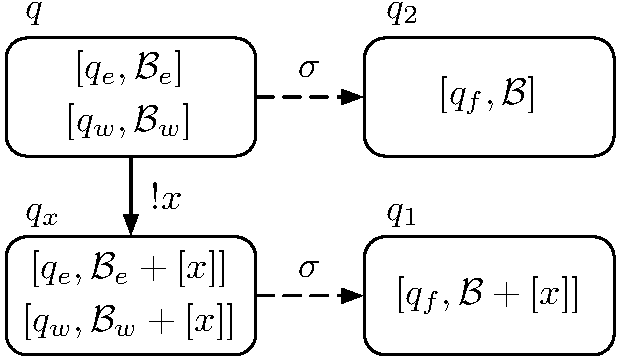
\includegraphics[scale=0.45]{diagnosis/covered}}}
\subfigure[hidden choice transition of \autoref{def:cfm}\label{fig:covered2}]{\makebox[0.49\textwidth]{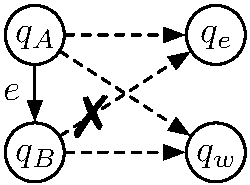
\includegraphics[scale=0.45]{diagnosis/covered2}}}
\caption{Illustrations for \autoref{lem:covered} and \autoref{def:cfm}.}
\label{fig:covered}
\end{figure}
%%%%%%%%%%%%%%%%%%%%%%%%%%%%%%%%%%%%%%%%%%%%%%%%%%%%%%%%%%%%%%%%%%%%%%%%%%%%%%

Each application of \autoref{lem:covered} identifies an $!x$-labeled transition from~$q$ to state $q_{x}$ from which a state $q_{1}$ is reached which contains a covered final state with a pending $x$-message, which is never received. For state~$q$, an alternative continuation to $q_{2}$ without an $!x$-transition is possible.

Hence, such a state $q_{x}$ should be considered critical, which yields the following definition of a blacklist for covered final states.




%%%%%%%%%%%%%%%%%%%%%%%%%%%%%%%%%%%%%%%%%%%%%%%%%%%%%%%%%%%%%%%%%%%%%%%%%%%%%%
\begin{definition}{Blacklist for covered final states}\label{def:cfm}%
Let, $q$, $q_x$, $q_1$, $q_2$, $q_e$, and $q_w$ as defined to be as in \autoref{lem:covered} and its proof (cf.~\autoref{fig:covered1}). We define the \define{blacklist for covered final states}, $\bl_{CFS}$, to contain exactly those states~$q_x$. Define the witness for a blacklisted state $q_x$, $W_{CFS}(q_x):=\{ q_A\xrightarrow{e}_{A} q_B \mid q_A\xrightarrow{*}q_w \wedge q_B\xrightarrow{*}q_w \wedge q_A\xrightarrow{*}q_e \wedge q_B\not\xrightarrow{*}q_e \}$, to contain all \define{hidden choice transitions} of $A$.
\end{definition}
%%%%%%%%%%%%%%%%%%%%%%%%%%%%%%%%%%%%%%%%%%%%%%%%%%%%%%%%%%%%%%%%%%%%%%%%%%%%%%

A covered final state is a situation which occurs in case a service automaton $A$ is composed to a partner. With the help of \autoref{lem:covered}, the blacklist for covered final states can be defined only by checking the states of $\TS^{0}_\mathit{red}(A)$ and paths in $\TS^{0}_\mathit{red}(A)$ and $A$. This can be realized during the construction $\TS^{0}_\mathit{red}(A)$ instead of analyzing paths in $A\oplus\TS^{0}_\mathit{red}(A)$. \Autoref{lem:covered} also allows for finding a set of \emph{hidden choice transitions} (see \autoref{fig:covered2}), which model a hidden decision as described in \autoref{sect:diagnosis:reasons}. These transitions can be the starting point to repair the service to avoid the covered final state.





%%%%%%%%%%%%%%%%%%%%%%%%%%%%%%%%%%%%%%%%%%%%%%%%%%%%%%%%%%%%%%%%%%%%%%%%%%%%%%%
\section{Diagnosis algorithm}\label{diagnosis:sect:algorithm}
%%%%%%%%%%%%%%%%%%%%%%%%%%%%%%%%%%%%%%%%%%%%%%%%%%%%%%%%%%%%%%%%%%%%%%%%%%%%%%%

With the definitions of the blacklists, we are finally able to define the subgraph $\TS^{0*}_k(A)$ (i.\,e., the counterexample for controllability of $A$) of $\TS_{k_\mathit{red}}(A)$ which only contains states which are not contained in any of the blacklists. Thereby, we ignore states which have become unreachable from the initial state.

%%%%%%%%%%%%%%%%%%%%%%%%%%%%%%%%%%%%%%%%%%%%%%%%%%%%%%%%%%%%%%%%%%%%%%%%%%%%%%
\begin{algorithm}[t!]
\restylealgo{boxed}
\SetVline
\caption{Blacklist-based diagnosis for uncontrollable services}
\label{alg:diagnosis}\footnotesize
\BlankLine
\KwIn{uncontrollable finite state service automaton $A$, message bound $k$}
\KwOut{diagnosis information, $\TS^{0*}_k(A)$}
\BlankLine
{calculate $\TS^{0}_\mathit{red}(A)$}

{derive $\bl_\mathit{DLL}$} from $\TS^{0}_\mathit{red}(A)$

{derive $\bl_\mathit{EMB}$} from $\TS^{0}_\mathit{red}(A)$

{derive $\bl_\mathit{CFS}$} from $\TS^{0}_\mathit{red}(A)$
\BlankLine
\eIf{$q_{0}$ is blacklisted}{
\If{$q_{0}\in\bl_\mathit{DLL}$}{
\ForEach{witness $q^*\in W_{DLL}(q_0)$}{
{\textbf{print} ``internal deadlock/livelock $q^*$ reachable without interaction''}
}
}
\If{$q_{0}\in\bl_\mathit{EMB}$}{
\ForEach{witness $m^*\in W_{EMB}(q_0)$}{
{\textbf{print} ``message bound of channel $m^*$ exceeded without interaction''}
}
}} {
\ForEach{nonblacklisted state $q$ reachable from $q_{0}$}{
\ForEach{waitstate $[q',\mathcal{B}]\in q$ with \smash{$q'\xrightarrow{e}_A q''$} and $q_e$ with \smash{$q\xrightarrow{e} q_e$}}{
\If{$q_e$ is blacklisted}{
\textbf{print} ``resolving waitstate $[q',\mathcal{B}]$ may reach a bad state''

\If{$q_{e}\in\bl_\mathit{DLL}$}{
\ForEach{witness $q^*\in W_{DLL}(q_e)$}{
\textbf{print} ``in $q_e$: internal deadlock/livelock $q^*$ reachable''
}
}
\If{$q_{e}\in\bl_\mathit{EMB}$}{
\ForEach{witness $m^*\in W_{EMB}(q_e)$}{
\textbf{print} ``in $q_e$: message bound of channel $m^*$ violated''
}
}
\If{$q_{e}\in\bl_\mathit{CFS}$}{
\textbf{print} ``in $q_e$: message $e$ may be left unreceived''

\ForEach{witness $[q_1,x,q_2]\in W_{CFS}(q_e)$}{
\textbf{print} ``hidden choice transition: $[q_1,x,q_2]$``
}
}
}
}
}
\textbf{print} subgraph $\TS^{0*}_k$ of $\TS_\mathit{red}^0(A)$ without blacklisted states
}
\end{algorithm}
%%%%%%%%%%%%%%%%%%%%%%%%%%%%%%%%%%%%%%%%%%%%%%%%%%%%%%%%%%%%%%%%%%%%%%%%%%%%%%

Algorithm~\ref{alg:diagnosis} combines the defined blacklists together with their witnesses and gives information for each detected problem. After a preprocessing phase (line 1--4) in which $\TS^{0}_\mathit{red}$ as well as the blacklists are calculated, the states of $\TS^{0}_\mathit{red}$ are analyzed. Thereby, two cases are differentiated: If already the initial state of $q_{0}$ is blacklisted, then the service can reach a bad state independently of a partner. Covered final states cannot occur in this setting. As a diagnosis information, the initial state $q_{0}$ and the respective problems are printed (line 5--11). The remainder of the algorithm (line~12--27) treats situations in which $\TS^{0*}_k$ is nonempty.

The diagnosis messages can be classified into the three categories (initial part~\acronym({I}), possible continuation~(\acronym{C}), and occurring problem~(\acronym{P})) as follows:
\begin{labeling}{(\acronym{C})}
\item[(\acronym{I})] line 27 prints the nonblacklisted subgraph $\TS^{0*}_k$,
\item[(\acronym{C})] line 16 prints a nonblacklisted waitstate whose resolution may reach a bad state,
\item[(\acronym{P})] line 8, 11, 19, 22, 24, and 26 print information about the problem which may be unavoidable after resolving the respective waitstate, including witnesses.
\end{labeling}

\enlargethispage*{\baselineskip}

The algorithm lists all problems which can occur if $\TS^{0*}_k$ is ``left'' by resolving a waitstate. If, for example, sending an $x$-message can result in a message bound violation \emph{and} yield an internal deadlock, then both problems are reported.




%%%%%%%%%%%%%%%%%%%%%%%%%%%%%%%%%%%%%%%%%%%%%%%%%%%%%%%%%%%%%%%%%%%%%%%%%%%%%%%
\subsection*{Implementation and experimental results}

The diagnosis has been implemented into the tool Wendy~\cite{LohmannW_2009_wendy}. In a special diagnosis mode, it constructs the reduced strategy from which the blacklists are generated.

The practical applicability of the diagnosis information is hard to measure and needs further investigation. To give an impression on the runtime and the sizes of the counterexamples, \autoref{tab:redsynthesis} lists results on synthesizing reduced strategies for the services we described in~\autoref{sect:background:experiment}. The reduced strategies consist only of a fraction of states and all can be calculated in less than a second. The nonblacklisted subgraph which is used as counterexample for controllability is a subgraph of the reduced synthesized strategy, so the numbers of \autoref{tab:redsynthesis} can be seen as an upper bound for the size of the counterexample.

%%%%%%%%%%%%%%%%%%%%%%%%%%%%%%%%%%%%%%%%%%%%%%%%%%%%%%%%%%%%%%%%%%%%%%%%%%%%%%
\begin{table}[tb]
\centering
\caption{Experimental results for reduced strategy synthesis using Wendy.}\medskip
\label{tab:redsynthesis}
\footnotesize
\begin{tabular*}{\textwidth}{@{\extracolsep{\fill}}lrrrrrr}
\toprule
& \multicolumn{3}{c}{most-permissive strategy} & \multicolumn{3}{c}{reduced strategy} \\ 
service & \multicolumn{1}{c}{$|Q_{\TS}|$} & \multicolumn{1}{c}{$|{\shortrightarrow}_{\TS}|$} & \multicolumn{1}{c}{time (sec)} & \multicolumn{1}{c}{$|Q_{\TS_\mathit{red}}|$} & \multicolumn{1}{c}{$|{\shortrightarrow}_{\TS_\mathit{red}}|$} & \multicolumn{1}{c}{time (sec)} \\ \midrule
Quotation &             $11{,}264$ & $145{,}811$ &   $3$ & $62$ & $77$ & $0$ \\
Deliver goods &          $1{,}376$ &  $13{,}838$ &   $2$ & $53$ & $82$ & $0$ \\ %daniela
{\scriptsize SMTP} protocol  & $20{,}818$ & $144{,}940$ &  $29$ & $62$  & $78$ & $0$ \\ %-m3
Car analysis &    $1{,}448$ &  $13{,}863$ &  $52$ & $108$ & $183$ & $1$ \\ %daniela
Identity card &      $1{,}536$ &  $15{,}115$ & $83$ & $259$ & $1{,}027$ & $1$ \\
Product order &    $57{,}996$ & $691{,}414$ & $303$ & $461$ & $938$ & $0$ \\ %-m2
\bottomrule
\end{tabular*}
\end{table}
%%%%%%%%%%%%%%%%%%%%%%%%%%%%%%%%%%%%%%%%%%%%%%%%%%%%%%%%%%%%%%%%%%%%%%%%%%%%%%


\Autoref{fig:diagnosis:example} depicts an uncontrollable service automaton and the diagnosis output of the tool Wendy. It consists of a graphical representation of the subgraph as well as a textual description of the problems and recommendations how to fix these issues. For instance, if the violation of a given message bound is the only detected problem, then the user is advised to restart the analysis with an increased message bound. The visualization of the counterexample generated by the diagnosis algorithm is in a very early state and needs to be tightly integrated to a service modeling tool. This integration is subject to future work and out of scope of this thesis.

%%%%%%%%%%%%%%%%%%%%%%%%%%%%%%%%%%%%%%%%%%%%%%%%%%%%%%%%%%%%%%%%%%%%%%%%%%%%%%
\begin{figure}[tb]
\centering
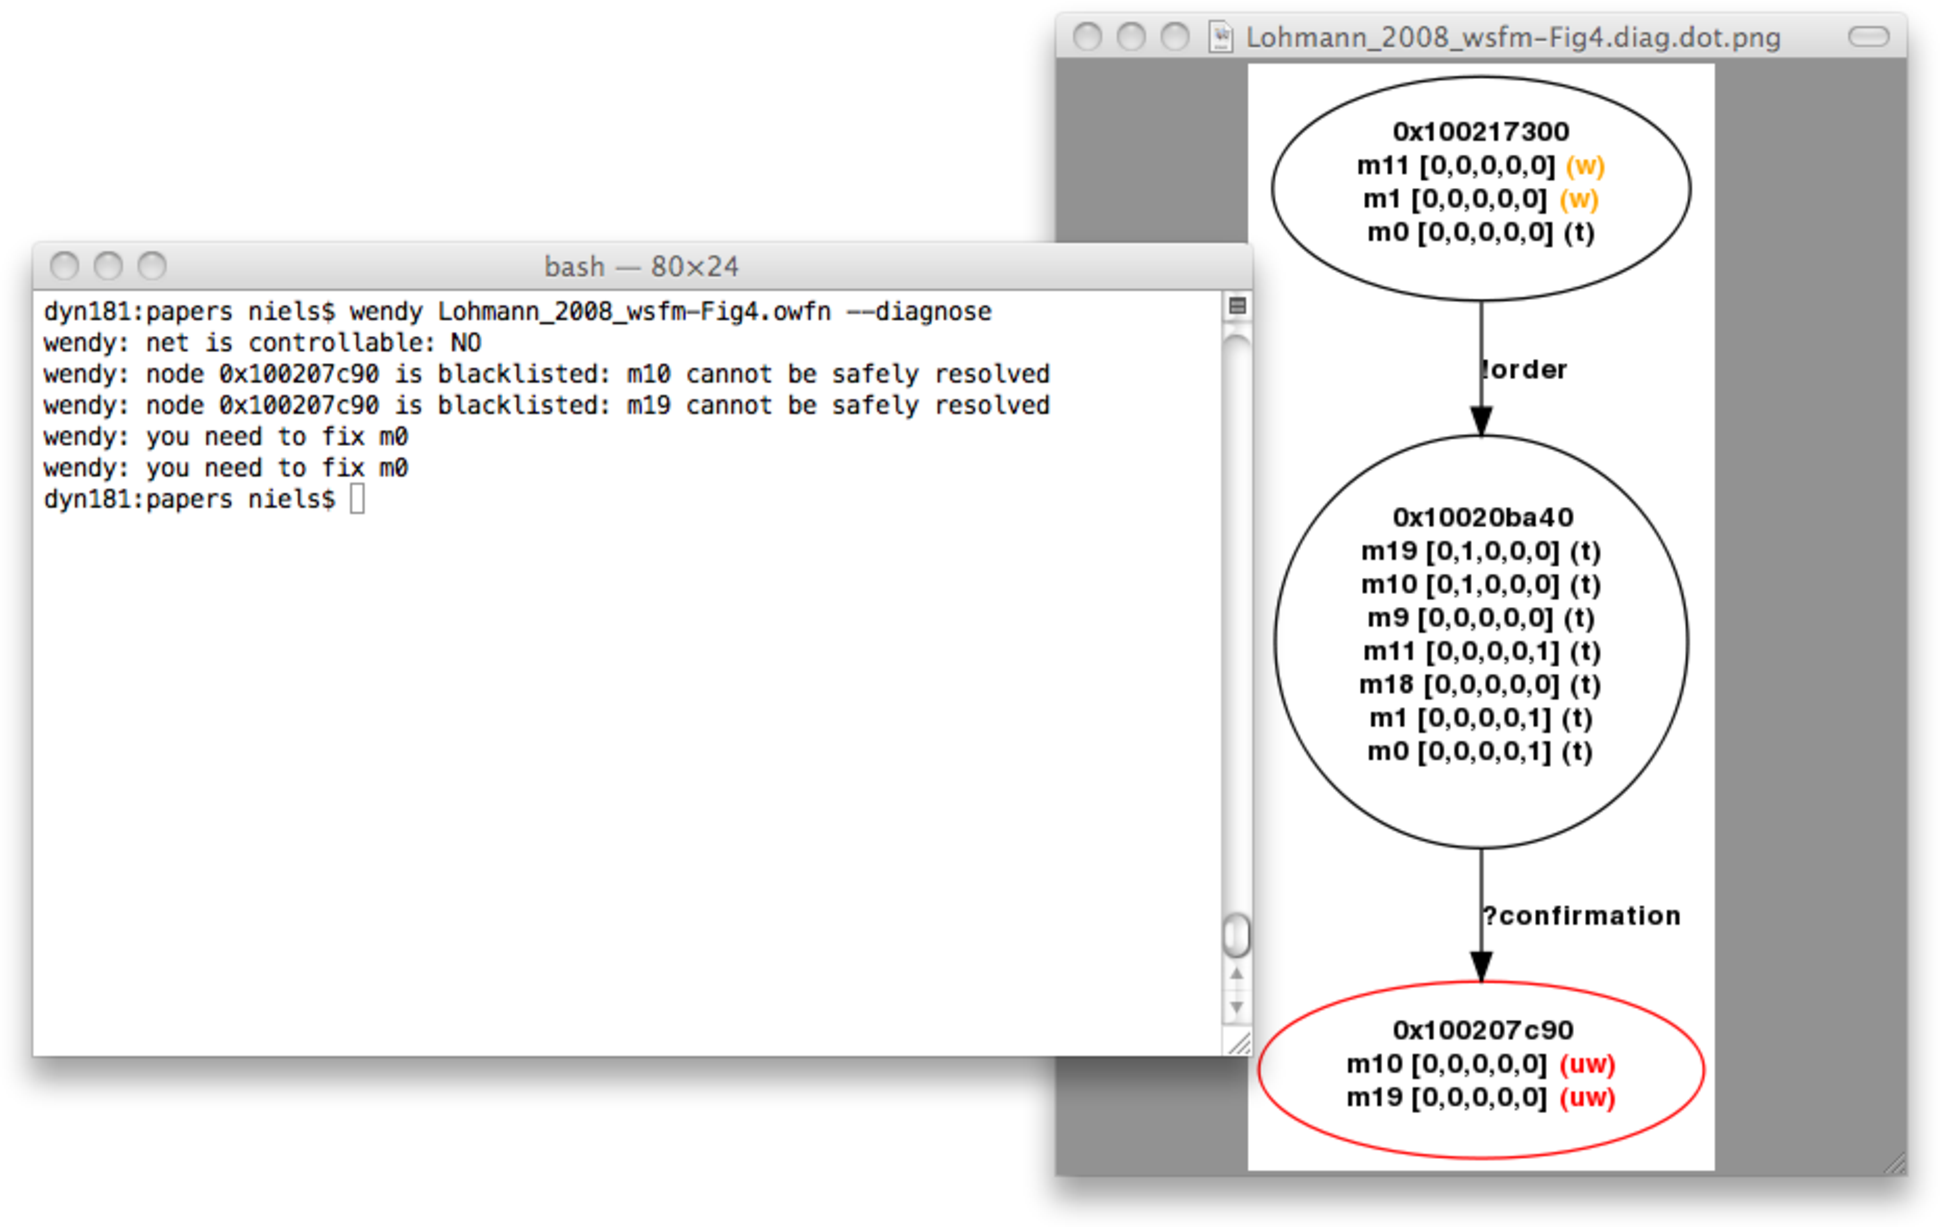
\includegraphics[width=0.8\textwidth]{diagnosis/wendydiag}
\caption{Diagnosis output of the tool Wendy.}
\label{fig:diagnosis:example}
\end{figure}
%%%%%%%%%%%%%%%%%%%%%%%%%%%%%%%%%%%%%%%%%%%%%%%%%%%%%%%%%%%%%%%%%%%%%%%%%%%%%%





%\enlargethispage*{\baselineskip}

%%%%%%%%%%%%%%%%%%%%%%%%%%%%%%%%%%%%%%%%%%%%%%%%%%%%%%%%%%%%%%%%%%%%%%%%%%%%%%%
\section{Conclusion}\label{sect:diagnosis:conclusion}
%%%%%%%%%%%%%%%%%%%%%%%%%%%%%%%%%%%%%%%%%%%%%%%%%%%%%%%%%%%%%%%%%%%%%%%%%%%%%%%

The generation of counterexamples greatly boosted the acceptance of model checking~\cite{ClarkeGD_1999_book} in the field of computer-aided verification. They present the reasons which make a model incorrect and therefore are as important as the verification procedure itself. However, the decision algorithm for controllability (cf.~\autoref{def:synthesis}) does not provide such counterexamples. In this chapter, we investigated uncontrollable service models and presented a variety of reasons why a service does not have any partners which interact in a compatible manner. We elaborated how a counterexample for controllability should be shaped to help the modeler understand the reasons which make a service uncontrollable. An algorithm to construct such a counterexample has been defined in terms of blacklists and has been prototypically implemented. The returned diagnosis information can be the starting point for corrections of the service toward controllability. We shall come back to this in \autoref{chap:correction}. The diagnosis algorithm can be directly used for refinements of controllability, for instance behavioral constraints (cf.~\autoref{chap:validation}), and is likely to be applicable to further extensions.

\medskip

Several aspects of diagnosing uncontrollable services remain subject of future work. First, service models usually stem from industrial specification languages, such as \acronym{WS-BPEL}. Hence, the retranslation of (automaton-related) diagnosis information back into \acronym{WS-BPEL} is a prerequisite to correlate the problems to the original model. Existing translations between service automata and \acronym{WS-BPEL}~\cite{Lohmann_2007_wsfm,LohmannK_2008_mod} could be extended to translate the necessary diagnosis information. In particular, a mapping between diagnosed bad states and activities in the original process could be challenging.

Second, the acceptance of the counterexamples needs to be further investigated. First experiments showed that especially hidden choices are often overlooked even by experienced service modelers. Nonlocality, asynchronous message exchange, and the absence of a concrete interaction partner are only a few of the reasons which make uncontrollable services hard to detect during modeling time.

Finally, further reduction techniques from \citet{Weinberg_2008_wsfm} may help to define a more compact counterexample for controllability. Reducing the size of the counterexample not only increases the understandability, but allows for faster calculation. This is crucial to be able to integrate the diagnosis algorithm into modeling tools. A constant analysis of a service model (\eg, each time the model is stored) helps to quickly correlate diagnosed problems to recent changes. For the soundness criterion, it is already possible to integrate verification techniques into industrial modeling tools~\cite{FahlandWJKLVW_2009_bpm} and verify the model constantly.
